\documentclass[11pt]{book}

%\usepackage[width=7.0in, height=9.0in, top=1.0in, papersize={8.5in,11in}]{geometry}
%\usepackage[pdftex]{graphicx}
%%\usepackage{datetime}
%\usepackage{anyfontsize}
%\usepackage{t1enc}
%\usepackage{verbatim}
%\usepackage{algorithm}
%\usepackage{algorithmic}
%\usepackage{framed}
%\usepackage{pdfpages}
%\usepackage{listings}
%\lstset{language=C}

\lstset{language=python,frame=ltrb,framesep=5pt,basicstyle=\normalsize,
 keywordstyle=\ttfamily\color{DarkRed},
%morecomment=[n][\textbf]{In\ [}{]\:},
%morecomment=[n][\textbf]{Out\ [}{]\:},
morecomment=[s][\color{blue}]{In\ [}{]\:},
morecomment=[s][\color{red}]{Out[}{]\:},
identifierstyle=\ttfamily\color{DarkBlue}\bfseries,
commentstyle=\color{DarkGreen},
stringstyle=\ttfamily,
showstringspaces=false,tabsize = 3}


\lstdefinelanguage{shell} {
commentstyle = \color{black},
keywordstyle = \color{black},
stringstyle = \color{black},
identifierstyle = \color{black},
morecomment=[s][\color{blue}]{In\ [}{]\:},
morecomment=[s][\color{red}]{Out[}{]\:},
 }

\pagestyle{empty}

%\usepackage{helvet}
\renewcommand{\familydefault}{\sfdefault}

\begin{document}

%{\fontsize{16}{16}\selectfont Sprint Report \#3}

\section*{Team Overview}
\hrulefill
\subsection*{Members}
Mackenzie Smith, Alex Nienhueser

\subsection*{Project Title}
Dahl Virtual Museum Tour

\subsection*{Company}
Dahl Arts Center


\section*{Sprint Report}
\hrulefill
\subsection*{Work Accomplished}
\begin{itemize}
\item On-Rails Tour as well as Free Moving Tour
\item Gathered test data on users experience in both movement modes
\item Converting pictures to Unreal textures
\item Placed each painting in its place
\item Fixed jittering issue with Oculus

\end{itemize}
\subsection*{Work Left}
\begin{itemize}
\item User documentation
\item Fix head rotation issue
\item Obtain missing art pieces from Dahl
\item Implement narration and text descriptions
\item Research into alternate environments
\end{itemize}

\section*{Movement and Testing}
In order to effectively move from painting to painting, a set of coordinates in the x,y,z plane were measured a certain distance away from the painting.  These sets of coordinates are then placed into an array in the Unreal Engine and with a forward arrow key press, the user will step to the next painting in the array; with each back press, the previous.  This was the best way that we came up with to achieve the on-rails feel by locking the positions into an array and using a linear interpolation function in Unreal, (lerp) to move between the positions.  These arrow keys will be mapped to the xbox 360 right and left buttons.

The testing that we did during this sprint involved anyone who wanted to participate.  We asked them to answer a few questions before trying out the Oculus where we tried to gauge their previous experience both with virtual reality and motion sickness.  Participants were asked to rate how easily they get motion sick on a scale from 1-10 with 10 being very easily. After this we then had them try on the Oculus and go through a few pictures in the on-rails mode, then in free movement.  After they were done, they filled out the remaining questions on the questionnaire. 

From our tests we gathered that on-rails movement causes less simulation sickness than the free movement.  In general the participants put a lower value for the on-rails than for free movement, using the same scale from 1-10.  This was expected due to the fact that Oculus recommends not having player controlled movement because of the fact that it causes more severe simulation sickness.

Finally we asked for any comments and suggestions about how we can improve the experience.  The most frequent suggestion was a movement speed setting, to increase or decrease movement speed both in on-rails and free movement.  This is something we will consider adding later in the project.  One other suggestion that is worth mentioning is the fact that in order to turn the player's body a full 360 degrees in the gallery, the user would have to turn all the way around in the physical world.  This detracts from the experience and we will be looking into how to fix that.

\section*{Client Interactions}
Most of this sprint was spent working on the gallery to implement each painting and get the lighting just right.  Our meetings with Dr. Adkins were few, only two, however communication via email has been the best way to communicate issues and thoughts about the project.  

We invited Dr. Adkins to our testing session in the McLaury building and we talked about some of the issues that came up with that, the resolution problem with the Oculus as well as the lack of paintings (which has been completed).  Apart from that he really enjoyed the experience and looks forward to the finished product.

The second interaction wasn't quite a meeting to discuss the project, it was more of a way to gain some insight into the art we are representing in the gallery.  Both Alex and Mack went to the Dahl on Wednesday, November 18th, to attend a talk given by the artist of the gallery, Arthur Amiotte.  Unfortunately we did not get to meet with him, but the stories he talked about gave insight into the paintings in the gallery.

\section*{Code Samples}

This is the addition to the on-rails movement system.  Notice the increment and decrement code blocks that have special cases to make the array of coordinates circular. 

\begin{figure}
\caption{The increment has the two plus signs, decrement with two minus signs}
\centering
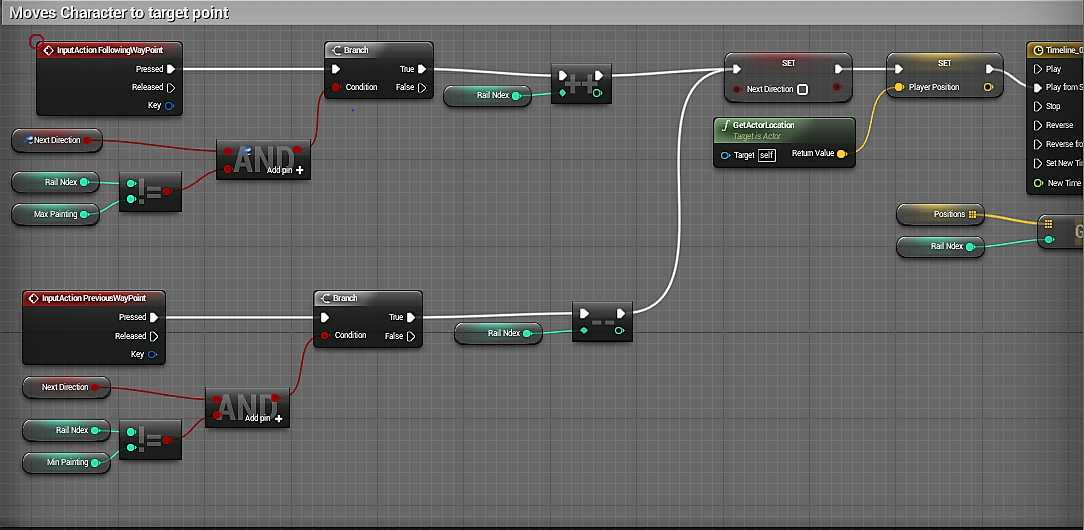
\includegraphics[scale=0.75]{WayMove1.png}
\end{figure}

\begin{figure}
\caption{Here you can see the lerp (mentioned before) function being called}
\centering
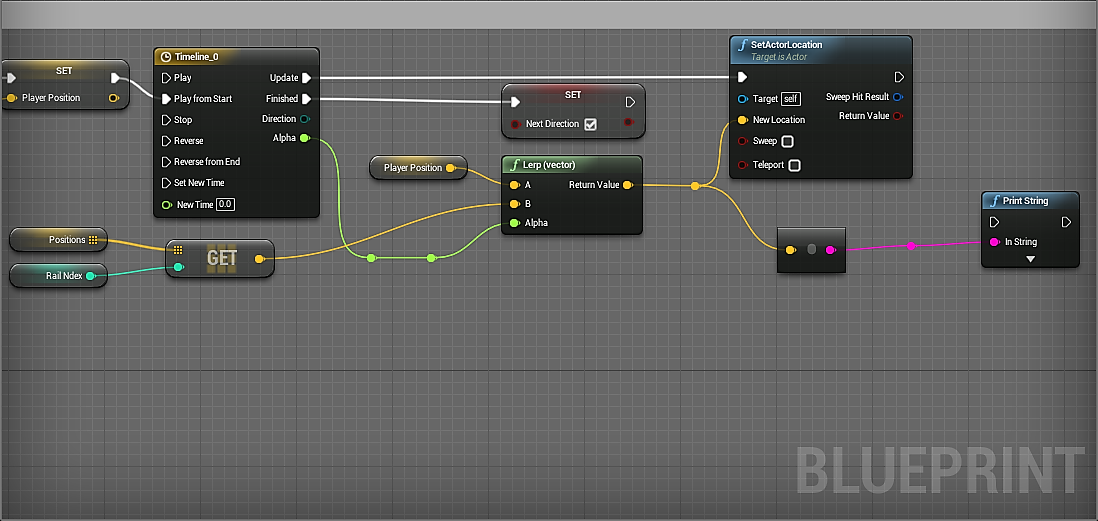
\includegraphics[scale=0.75]{WayMove2.png}
\end{figure}

\begin{figure}
\caption{This is only a section of the array containing the coordinates}
\centering
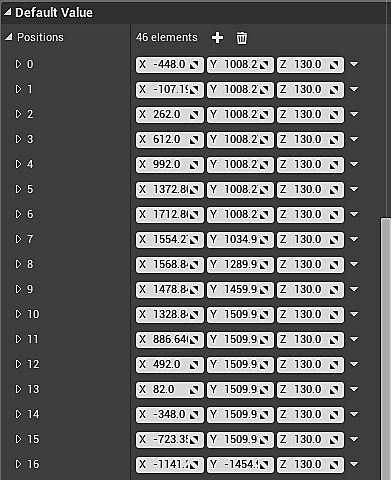
\includegraphics[scale=1.0]{Waypoint.png}
\end{figure}


\section*{Problems Encountered}
\begin{enumerate}
\item There is an issue with texturing the rounded corners of the gallery because of the way we implemented them.

\item As mentioned in the Movement and Testing section, an issue with turning beyond 180 degrees, which requires mouse movement.  

\item Although we requested the pictures that were missing in the original picture set, there are still pictures missing from our virtual gallery that are in the real one.
\end{enumerate}




\end{document}